\documentclass[12pt,a4paper]{article}
\usepackage[T2A]{fontenc}
\usepackage[utf8]{inputenc}
\usepackage[russian]{babel}
\usepackage{amsmath}
\usepackage{geometry}
\usepackage{fancyvrb}
\usepackage{graphicx}
\geometry{left=2cm,right=2cm,top=2cm,bottom=2cm}
\begin{document}
\pagestyle{empty}
\begin{center}
    {\fontsize{12pt}{14pt}\selectfont
        МИНИСТЕРСТВО НАУКИ И ВЫСШЕГО ОБРАЗОВАНИЯ\\
        РОССИЙСКОЙ ФЕДЕРАЦИИ\\
        Федеральное государственное бюджетное образовательное учреждение\\
        высшего образования\\
        \textbf{АДЫГЕЙСКИЙ ГОСУДАРСТВЕННЫЙ УНИВЕРСИТЕТ}\\
    }
    \vspace{0.3cm}
    {\fontsize{12pt}{14pt}\selectfont
        Институт точных наук и цифровых технологий\\
        Кафедра автоматизированных систем обработки информации и\\
        управления\\
    }
\end{center}
\vspace{4.5cm}
\begin{center}
    {\fontsize{14pt}{16pt}\selectfont ОТЧЕТ ПО ПРАКТИКЕ\\}
    \vspace{0.5cm}
    {\fontsize{16pt}{18pt}\selectfont \textbf{Программная реализация численного метода}\\}
   {\fontsize{14pt}{16pt}\selectfont \textit{Вариант 1. Интерполяция функции с использованием многочлена Лагранжа}\\}
    \vspace{0.8cm}
    {\fontsize{12pt}{14pt}\selectfont 1 курс, группа УТС\\}
\end{center}
\vspace{3cm}
\hfill
\begin{minipage}{0.48\textwidth}
    {\normalsize Выполнил:\\
    \underline{\hspace{3.5cm}} П. И. Осауленко\\
    «\underline{\hspace{0.8cm}}» \underline{\hspace{2.2cm}} 2026 г.\\
    \vspace{0.6cm}
    Руководитель:\\
    \underline{\hspace{3.5cm}} С. В. Теплоухов\\
    «\underline{\hspace{0.8cm}}» \underline{\hspace{2.2cm}} 2026 г.}
\end{minipage}
\vfill 
\begin{center}
    {\normalsize Майкоп, 2026 г.}
\end{center}
\newpage
\section{Задание}

Интерполировать функцию, используя многочлен Лагранжа.
Количество точек задается пользователем.
Пользователь вводит координаты точек $(x_i,y_i)$ и значение аргумента $X$, для которого необходимо вычислить значение интерполяционного многочлена.

\section{Теоретическая часть}

Интерполяционный многочлен Лагранжа применяется для построения функции, проходящей через заданный набор точек.

Пусть заданы точки

\[
(x_0,y_0),(x_1,y_1),...,(x_n,y_n).
\]

Тогда значение интерполяционного многочлена определяется выражением

\[
L(x)=\sum_{i=0}^{n}y_i
\prod_{\substack{j=0\\j\neq i}}^{n}
\frac{x-x_j}{x_i-x_j}.
\]

Каждый базисный многочлен равен единице в своей точке и нулю во всех остальных. Благодаря этому построенный многочлен проходит через все заданные точки.

\section{Реализация и контроль ввода}

Программа написана на языке C++.

Для обеспечения корректной работы реализованы следующие проверки:

\begin{itemize}
\item проверка количества вводимых точек;
\item проверка корректности ввода координат точек;
\item проверка отсутствия одинаковых значений $x$;
\item проверка корректности ввода значения $X$.
\end{itemize}

После успешного ввода данных вычисляется значение интерполяционного многочлена Лагранжа в заданной точке.

\newpage

\section{Исходный код программы}

Ниже представлен полный исходный код разработанной программы.

\begin{Verbatim}[frame=single,numbers=left,tabsize=4]
#include <iostream>
#include <vector>
#include <clocale>

using namespace std;

double Lagrange(vector<double> x, vector<double> y, double X) {
    double result = 0;

    for (int i = 0; i < x.size(); i++) {
        double term = y[i];

        for (int j = 0; j < x.size(); j++) {
            if (i != j) {
                term *= (X - x[j]) / (x[i] - x[j]);
            }
        }

        result += term;
    }

    return result;
}

int main() {
    setlocale(LC_ALL, "Russian");

    int n;

    while (true) {
        cout << "Введите количество точек (не меньше 2): ";

        if (cin >> n && n >= 2) {
            break;
        }
        else {
            cout << "Количество точек должно быть целым числом не меньше 2." << endl;
            cin.clear();
            cin.ignore(1000, '\n');
        }
    }

    vector<double> x(n);
    vector<double> y(n);

    cout << endl;
    cout << "Введите координаты точек:" << endl;

    for (int i = 0; i < n; i++) {

        while (true) {
            cout << "x[" << i << "] = ";

            if (cin >> x[i]) {
                break;
            }
            else {
                cout << "Введено не число." << endl;
                cin.clear();
                cin.ignore(1000, '\n');
            }
        }

        while (true) {
            cout << "y[" << i << "] = ";

            if (cin >> y[i]) {
                break;
            }
            else {
                cout << "Введено не число." << endl;
                cin.clear();
                cin.ignore(1000, '\n');
            }
        }
    }

    for (int i = 0; i < n; i++) {
        for (int j = i + 1; j < n; j++) {

            if (x[i] == x[j]) {
                cout << endl;
                cout << "Ошибка! Значения x должны быть различными." << endl;
                return 0;
            }

        }
    }

    double X;

    while (true) {
        cout << endl;
        cout << "Введите значение X для интерполяции: ";

        if (cin >> X) {
            break;
        }
        else {
            cout << "Введено не число." << endl;
            cin.clear();
            cin.ignore(1000, '\n');
        }
    }

    double result = Lagrange(x, y, X);

    cout << endl;
    cout << "L(" << X << ") = " << result << endl;

    return 0;
}
\end{Verbatim}

\newpage

\section{Результат работы программы}

\begin{figure}[h!]
\centering
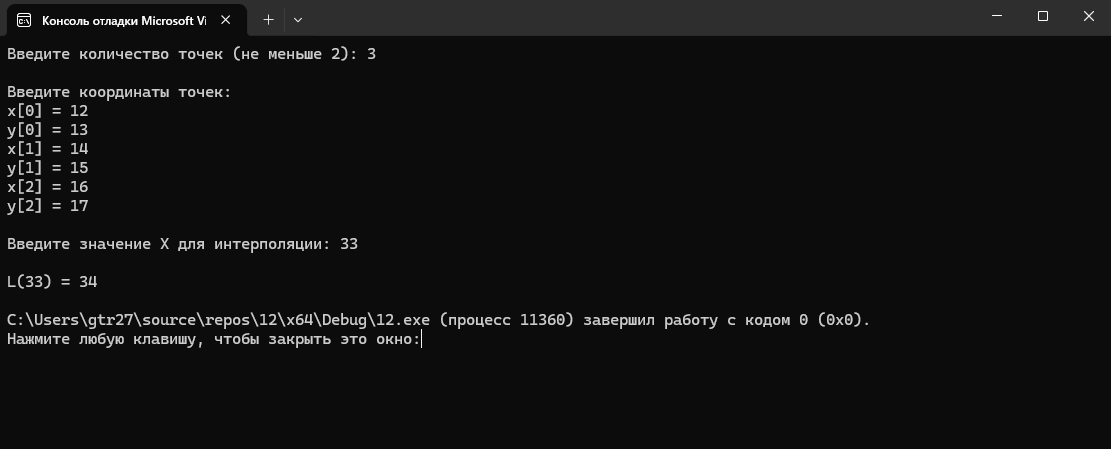
\includegraphics[width=0.8\textwidth]{screenshot.png}
\caption{Результат работы программы}
\end{figure}

\end{document}
